%===============================================================================
\chapter{Identifica��o de sistemas n�o lineares}
\label{chapter:nlin_si_ident}
%===============================================================================
% idea: Colocar aqui neste capitulo todas as defini��es genericas sobre 
% n�o linearidades. coisas que na� sao relacionadas com o que eu vou fazer, ou que n�o
% sao conseguencia dela.
%
% lineariza��o: Descrever que muitas aplica�oes de identifica��o de sis nonlineares �
% linearizar ele em torno de um ponto. que isso ja eh bom suficiente.
%
% Models: Descrever os tipos de modelos para descrever sistemas nao lineares. Aqui 
% da para escrever bastante coisa. existem muito tipo de modelos para isso.
%
% Algoritmos: aqui vai o algoritmo do aguirre para modelos racionais. Talvez fosse de
% pensar em colcar isso no capitulo com minhas contribui��es? acho que nao .. referencio isso
% no meu capitulo.
%
% Conclus�es: Resumo do que foi visto aqui 
%===============================================================================
%===============================================================================
\section{Conceitos b�sicos}
\label{sec:nlin_si_basic}
%===============================================================================

%===============================================================================
\subsection{Lineariza��o}
\label{sec:nlin_si_basic_linearization}
%===============================================================================
% Khalil
% ljng 		142
% Aguirre

Talvez o mais comum uso de sistemas lineares variantes no tempo esta relacionado
a lineariza��o de sistema n�o lineares em torno de uma trajet�ria. Suponha que
o sistema n�o linear � descrito por:\cite{ljung}

\begin{equation}
\left\{\begin{matrix}
x(k+1) = f(x(k),u(k))+r(x(k),u(k))w(k)\\ 
y(k)  = h(x(k))+m(x(k),u(k))\upsilon (k)
\end{matrix}\right.
\label{eq:nl_linearization_sys}
\end{equation}

Existem duas b�sicas limita��es para sistemas linearizados. Primeiro que a lineariza��o
� uma aproxima��o ao redor do ponto de opera��o, ele pode prever apenas o comportamento
nesta localidade do sistema e n�o o comportamento global. Segundo as din�micas
de sistemas n�o lineares s�o muito mais ricas que as de sistemas lineares. Existem alguns
fen�menos {\it{essenciais}}, n�o lineares, que n�o conseguem ser descritos ou
preditos por modelos lineares, estes s�o: \cite{khalil}

\renewcommand{\labelitemi}{$\bullet$}
\begin{itemize}

\item Tempo de fuga finito

O estado de um sistema linear inst�vel tende ao infinito na medida que o tempo 
tende ao infinito. Um sistema n�o linear est�vel, entretanto, pode ir para o
infinito em um tempo finito.


\item M�ltiplos pontos de equil�brios isolados

Um sistema linear tem apenas um ponto de equil�brio. Desta forma, este sistema pode
ter apenas um ponto do espa�o de estados que atraem o estado do sistema, independentemente
do estado inicial. Um sistema n�o linear pode ter mais de um ponto de equil�brio isolado. 
Desta forma o estado do sistema pode convergir para um destes equil�brios ou outro,
dependendo do estado inicial do sistema.

\item Ciclos limites

Para um sistema linear e invariante no tempo oscilar ele deve ter um par de autovalores
sobre o eixo imagin�rio, o que � uma condi��o n�o robusta praticamente imposs�vel de manter
na presen�a de perturba��es. Mesmo que isso seja poss�vel de manter, a amplitude da 
oscila��o depender� das condi��es iniciais do sistema. Na vida real, oscila��es est�veis
s�o atingidas com sistemas n�o lineares. Alguns sistemas possuem oscila��es com
amplitude e frequ�ncia constantes, independente das condi��es iniciais. Chama-se isso de
ciclos limites.

\item Sub harm�nicas, harm�nicas ou quase peri�dicas oscila��es

Um sistema linear est�vel sobre uma entrada peri�dica produz uma sa�da na mesma frequ�ncia.
Sistemas n�o lineares alimentados por sinais peri�dicos podem oscilar com frequ�ncias que
podem ser sub m�ltiplos ou m�ltiplos da frequ�ncia de entrada.

\item Caos

Um sistema n�o linear pode ter um espa�o de estados mais complexo que seu comportamento n�o 
pode ser descrito por oscila��es peri�dicas, ou quase peri�dicas oscila��es. Este comportamento
normalmente � conhecido como caos. Alguns destes movimentos ca�ticos exibem comportamento
rand�mico, independentemente da natureza do sistema.

\item M�ltiplos modos de comportamento

� comum para um sistema n�o linear exibir dois ou mais modos de comportamento distintos.
\end{itemize}










%===============================================================================
\section{Modelos para sistemas n�o lineares}
\label{sec:nl_models}
%===============================================================================

\cite{CampiSacvaresi-vrft_nonlinear}

%===============================================================================
\subsection{Modelos de Wiener e Hammerstein}
\label{sec:nl_models_wiener_hammerstein}
% Aguirre: 334
% ljung 143
%===============================================================================

Em uma situa��o onde a din�mica do sistema pode ser bem descrita por um sistema linear, 
mas existem algumas n�o linearidades est�ticas atreladas a entrada e/ou a sa�da.
Este ser� o caso de atuadores serem n�o lineares como por exemplo: devido a satura��o, 
ou se o sensor tem caracter�sticas n�o lineares. 

Um modelo com n�o linearidades na entrada � chamado de {\it{modelo de Hammerstein}} e 
para n�o linearidades na sa�da chama-se {\it{modelo de Wiener}}. \cite{ljung}

Considere o sistema apresentado em \eqref{eq:nl_linearization_sys} e o caso de 
Hammerstein, tem-se que a fun��o est�tica n�o linear $f(\cdot)$ pode ser parametrizado
tanto em termos de par�metros f�sicos, como ponto ou n�vel de satura��o, como pode
ser parametrizado por modelo caixa preta.

Na Figura (\ref{fig:nl_models_hammerstein_wiener}) observa-se o diagrama de bloco para os modelos
de Hammerstein e Wiener.


\begin{figure}[htbp]
\center
\scalebox{1} % Change this value to rescale the drawing.
{
	\begin{pspicture}(0,-1.4)(8.949375,1.4)
		\psline[linewidth=0.04cm,arrowsize=0.08cm 2.0,arrowlength=1.4,arrowinset=0.4]{->}(0.0,0.8)(1.2,0.8)
		\psframe[linewidth=0.04,dimen=outer](3.4,1.4)(1.2,0.2)
		\psline[linewidth=0.04cm,arrowsize=0.08cm 2.0,arrowlength=1.4,arrowinset=0.4]{->}(3.4,0.8)(4.6,0.8)
		\psframe[linewidth=0.04,dimen=outer](6.8,1.4)(4.6,0.2)
		\psline[linewidth=0.04cm,arrowsize=0.08cm 2.0,arrowlength=1.4,arrowinset=0.4]{->}(6.8,0.8)(8.0,0.8)
		\psline[linewidth=0.04cm,arrowsize=0.08cm 2.0,arrowlength=1.4,arrowinset=0.4]{->}(0.0,-0.8)(1.2,-0.8)
		\psframe[linewidth=0.04,dimen=outer](3.4,-0.2)(1.2,-1.4)
		\psline[linewidth=0.04cm,arrowsize=0.08cm 2.0,arrowlength=1.4,arrowinset=0.4]{->}(3.4,-0.8)(4.6,-0.8)
		\psframe[linewidth=0.04,dimen=outer](6.8,-0.2)(4.6,-1.4)
		\psline[linewidth=0.04cm,arrowsize=0.08cm 2.0,arrowlength=1.4,arrowinset=0.4]{->}(6.8,-0.8)(8.0,-0.8)
		\usefont{T1}{ptm}{m}{n}
	\rput(0.489375,1.11){u(t)}
	\usefont{T1}{ptm}{m}{n}
	\rput(3.900625,1.11){f(u(t))}
	\usefont{T1}{ptm}{m}{n}
	\rput(7.299375,1.11){y(t)}
	\usefont{T1}{ptm}{m}{n}
	\rput(5.6226563,0.91){Modelo}
	\usefont{T1}{ptm}{m}{n}
	\rput(5.5264063,0.51){Linear}
	\usefont{T1}{ptm}{m}{n}
	\rput(2.2226562,-0.69){Modelo}
	\usefont{T1}{ptm}{m}{n}
	\rput(2.1264062,-1.09){Linear}
	\usefont{T1}{ptm}{m}{n}
	\rput(2.180625,0.71){f()}
	\usefont{T1}{ptm}{m}{n}
	\rput(5.580625,-0.89){f()}
	\usefont{T1}{ptm}{m}{n}
	\rput(7.949375,-0.49){y(t)=f(z(t))}
	\usefont{T1}{ptm}{m}{n}
	\rput(0.489375,-0.49){u(t)}
	\usefont{T1}{ptm}{m}{n}
	\rput(3.876875,-0.49){z(t)}
	\end{pspicture} 
}
\caption{Acima: modelo de Hammerstein. Abaixo: Modelo de Wiener.}
\label{fig:nl_models_hammerstein_wiener}
\end{figure}

%===============================================================================
\subsection{Serie de Volterra}
\label{sec:nl_models_volterra}
% Aguirre 334
%===============================================================================

Um sistema n�o linear pode ser descrito pela serie de Volterra \eqref{eq:nl_models_volterra}:

\begin{equation}
y(t)=\sum_{j=1}^{\infty}\int_{-\infty}^{\infty}\cdots \int_{-\infty}^{\infty}
h_j(\tau_1, ... ,\tau_j) \prod_{i=1}^{j}u(t-\tau_i)d\tau_i
\label{eq:nl_models_volterra}
\end{equation}

Onde $h_j$ s�o generaliza��es n�o lineares da resposta ao impulso $h_1(t)$ . Para
um sistema linear com $j=1$ a equa��o de Volterra se reduz a integral de convolu��o.
\cite{aguirre}

Grande dificuldade de utilizar a serie de Volterra \eqref{eq:nl_models_volterra} � que
at� para sistemas pouco n�o lineares, o numero de par�metros a estimar � grande. Isso
se d� pelo fato da s�rie tentar explicar a sa�da do sistema apenas baseado nos valores
da entrada deste.

%===============================================================================
\subsection{Fun��es Radiais de Base}
\label{sec:nl_models_radiais}
% Aguirre 337
%===============================================================================

Fun��es radiais de base ({\it{RBF - Radial basis functions}} s�o mapeamentos do tipo:

\begin{equation}
f(y)-w_0+\sum_{i}w_i \phi (\left \| y-c_i \right \|)
\label{eq:nl_models_rbf}
\end{equation}

Sendo que $y \in \mathbb{R}^{d_e}$ ($d_e$ � conhecido como dimens�o de imers�o),
$\left \| \cdot \right \|$ � a norma euclidiana, $w_i \in \mathbb(R)$ s�o pesos, 
$c_i \in \mathbb{R}^{d_e}$ s�o centros e $\phi(\cdot):\mathbb{R}^+ \to \mathbb{R}$ 
� uma fun��o, normalmente escolhida a priori, como por exemplo: \cite{aguirre}

\begin{equation}
\phi(\left \| y-c_i \right \|)= exp\left ( -\frac{\left \| y-c_i \right \|^2}{\sigma_i^2} \right )
\nonumber
\end{equation}

Outras fun��es de base usadas s�o apresentadas na Tabela \ref{table:nl_models_rbf}

\begin{table*}[htbp]
\begin{center}
\caption{Algumas fun��es Radiais de base comumente usadas.}
\label{table:nl_models_rbf}
\begin{tabular}{ll}
\hline
        Nome & Fun��o   \\
\hline
        Multi quadr�tica inversa  & $\phi(r)=(r^2+\sigma ^2)^{-1/2}$ \\ 
        Linear                    & $\phi(r)=r$                      \\ 
        C�bica                    & $\phi(r)=r^3$                    \\ 
        Multiquadr�tica           & $\phi(r)=\sqrt{r^2+\sigma^2}$    \\ 
        {\it{Thin - plate spline}} & $\phi(r)=r^2\; \text{log}(r)$   \\ 
\hline
\end{tabular}
\end{center}
\end{table*}

Sendo que $r=\left \| y-c_i \right \|$ e $\sigma$ definem a largura do chap�u no caso de
fun��es gausianas e das multiquadr�ticas, como pode ser visto na figura (\ref{fig:nl_models_rbf}).

\begin{figure}[htbp]
	\center
	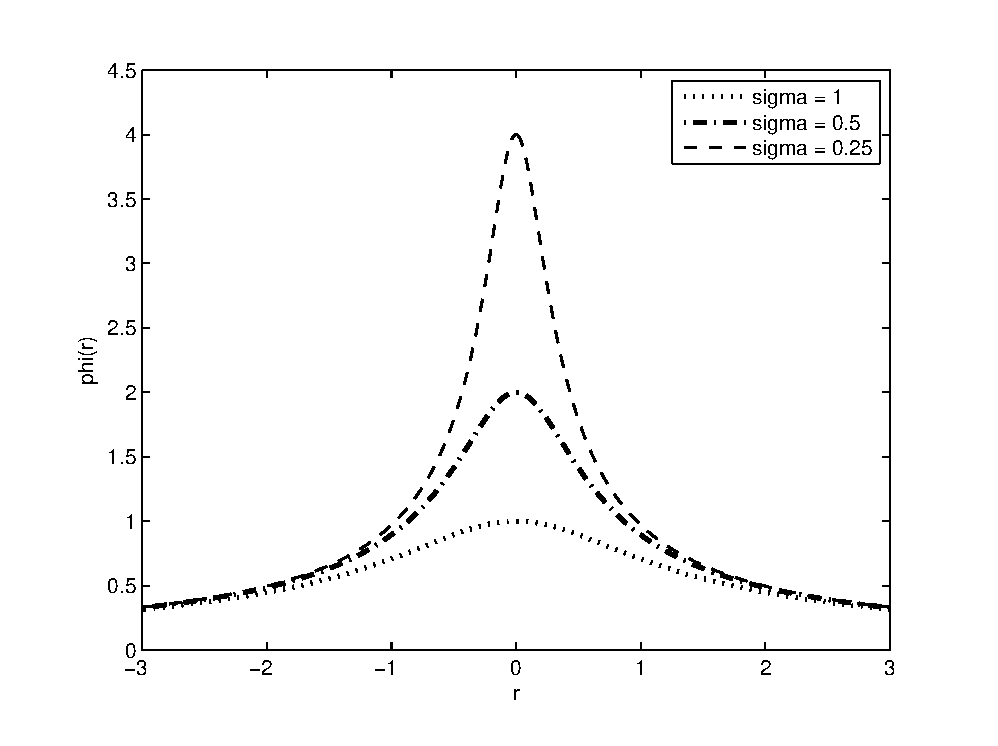
\includegraphics[width=0.8\columnwidth]{figures/nl_models_rbf.eps}
	\caption{Fun��o multiquadr�ticas inversa para alguns valores de $\sigma$.}
	\label{fig:nl_models_rbf}
\end{figure}

Este tipo de representa��o tem boas propriedades locais e pode ser interpretada como 
uma t�cnica de interpola��o global. Fun��es radiais de base s�o casos particulares
de redes neurais, porem neste caso lineares nos parametros $w_i$.\cite{aguirre} 

No contexto de identifica��o de sistemas � comum adicionar termos auto-regressivos
lineares, bem como termos de entrada � equa��o \eqref{eq:nl_models_rbf} resultando em:

\begin{equation}
y(k)=w_0 + \sum_{i}w_i \phi(\left \| \mathbf{y}(k-1)-c_i \right \|)+\sum_{i=1}^{n_y}a_i y(k-i)+\sum_{i=1}^{n_u}b_i u(k-i)+e(k)
\nonumber
\end{equation}

Sendo $\mathbf{y}(k-1)=\begin{bmatrix}
y(k-1) & ... & y(k-n_y) & u(k-1) & ... & u(k-n_u)
\end{bmatrix}$.

%===============================================================================
\section{Modelos NARMAX}
\label{sec:nl_models_narmax}
% Aguirre 343
%===============================================================================

Os modelos {\it{NARX}} (do termo ingles {\it{nonlinear autoregressive model with
exogenous variables}}) s�o modelos discretos no tempo que caracterizam o valor da 
sa�da em fun��o dos valor passados da entrada e sa�da. Algumas vezes, para evitar 
a polariza��o da estimativa dos parametros adiciona-se termos do ruido no modelo.
Quando isso � feito o modelo passa a ser chamado de um modelo {\it{NARMAX}} (do
termo ingles {\it{nonlinear autoregressive moving average model with exogenous
variables}}) que pode ser representado pla equa��o \eqref{eq:nl_model_narmax}. 
\cite{aguirre}

\begin{eqnarray}\nonumber
y(t)&=&F [ y(t-1), ..., y(t-n_y), u(t-1), ... , u(t-n_u),\\
&&  e(t),e(t-1), ... , e(t-n_e) ]
\label{eq:nl_model_narmax}
\end{eqnarray}

%\begin{equation}
%y(t)=F\left [ y(t-1), ..., y(t-n_y), u(t-1), ... , u(t-n_u), e(t),e(t-1), ... , e(t-n_e) \right ]
%\label{eq:nl_model_narmax}
%\end{equation}

Onde $e(t)$ � o ruido e $n_e$ � o maior atraso no modelo do ruido. O modelo apresentado
em \eqref{eq:nl_model_narmax} � bastante gen�rico, caracterizando uma dificuldade 
para sua utiliza��o. A caracteriza��o da equa��o $F$ geralmente � feita pelas 
representa��es polinomial e racional. Um modelo polinomial {\it{NARMAX}} sem atraso
puro de tempo tem a forma apresentada em \eqref{eq:nl_model_narmax_pol}.

\begin{equation}
y(t)=\sum_{i}c_i \prod_{j=1}^{n_y}y(t-j) \prod_{r=1}^{n_u}u(t-r) \prod_{q=0}^{n_e}e(t-q)
\label{eq:nl_model_narmax_pol}
\end{equation}

Os modelos polinomiais {\it{bilineares}} s�o casos particulares do modelo polinomial 
\eqref{eq:nl_model_narmax_pol} quando todos os termos n�o lineares s�o do tipo 
$y(t-i)u(t-j), \; \forall i,j$. \cite{aguirre}

Modelos racionais s�o formados pela raz�o entre dois polinomios \eqref{eq:nl_model_narmax_rat}.

\begin{equation}
y(t)=\frac{\sum_{i}c_i \prod_{j=1}^{n_y}y(t-j) \prod_{r=1}^{n_u}u(t-r) \prod_{q=0}^{n_e}e(t-q)}
{\sum_{i}c_i \prod_{j=1}^{n_y}y(t-j) \prod_{r=1}^{n_u}u(t-r) \prod_{q=0}^{n_e}e(t-q)} + e(t)
\label{eq:nl_model_narmax_rat}
\end{equation}

Em fun��o de terem uma estrutura mais floxivel, os modelos racionais opdem vir a ser
mais eficientes na modelagem de certos sistemas quando comparados com modelos polinomiais.
Entretanto, os modelos racionais s�o mais sens�veis ao ruido. \cite{aguirre}

%===============================================================================
\subsection{Modelo polinomial NARMAX}
\label{sec:nl_models_narmax_pol}
% Aguirre 343
%===============================================================================
Com rela��o ao modelo generico polinomial {\it{NARMAX}} apresentado em \eqref{eq:nl_model_narmax_pol}
duas considera��es ser�o levadas em conta:

\begin{enumerate}
\item O sistema tem um atraso puro de tempo $\tau _d$ 
\item Nenhum termo cujo parametro tenha que ser estimado pode depender de $e(t)$.
\end{enumerate}

A segunda considera��o implica em tornar $F$ independente de $e(t)$. O que equivale a dizer
que $q=1$ em \eqref{eq:nl_model_narmax_pol} resultando em  \eqref{eq:nl_model_narmax_pol_espec}.

\begin{eqnarray}\nonumber
y(t) &=& F[ y(t-1), ..., y(t-n_y), u(t-\tau_d), ..., u(t-\tau_d-n_u+1),\\
&& e(t-1), ..., e(t-n_e)] +e(t)
\label{eq:nl_model_narmax_pol_espec}
\end{eqnarray}

Sendo que $e(t)$ indica que todos os efeitos n�o podem ser bem representados por 
$F^l\left [ \cdot  \right ]$, � uma fun��o polinomial de $y(t)$, $u(t)$ e 
$e(t)$ com grau de n�o linearidade $l\in \mathbb{N}$. Portanto a parte 
n�o deterministica de \eqref{eq:nl_model_narmax_pol_espec} pode ser espandida como
um somat�rio de termos com grau de n�o linearidade variando de $1 \le m \le l$. 
Assim sendo, cada termo de grau $m$ poder� conter um falor de grau $p$ do tipo $y(t-i)$
e um fator de grau $(m-p)$ do tipo $u(t-i)$ sendo multiplicado por um parametro representado 
por $c_{p,m-p}(n_1, ..., n_m$. Resultando em: \cite{aguirre}

\begin{equation}
y(t)=\sum_{m=0}^{l}\sum_{p=0}^{m}\sum_{n1, n_m}^{n_y, n_u}c_{p,m-p}(n_1,...,n_m)\prod_{i=1}^{p}y(t-n_i)\prod_{i=p+1}^{m}u(t-n_i)
\nonumber
\end{equation}


%===============================================================================
\subsection{Modelo Racional NARMAX}
\label{sec:nl_models_narmax_rat}
% Aguirre 345
%===============================================================================

Um modelo racional {\it{NARMAX}} tem a seguinte forma geral apresentada em 
\eqref{eq:nl_model_narmax_rat} e de forma simplificada como apresentado em
\eqref{eq:nl_model_narmax_rat_simp}.

\begin{equation}
y(k)=\frac{a(\Upsilon)}{b(\Upsilon)}+e(t)
\label{eq:nl_model_narmax_rat_simp}
\end{equation}

Onde:

\begin{equation}
\Upsilon=\left \{ y(t-1), ..., y(t-n_y), u(t-1), ..., u(t-n_u), e(t-1), ..., e(t-n_e)\right \}
\nonumber
\end{equation}

No modelo apresentado em \eqref{eq:nl_model_narmax_rat}, as fun��es $a(\Upsilon)$ e $b(\Upsilon)$
s�o polinomios, mas poderiam ser quaisquer fun��es. Assumindo que o modelo � formado pela raz�o de
dois polinomios, � conveniente definir o numerador e denominador de \eqref{eq:nl_model_narmax_rat}
como em \eqref{eq:nl_model_narmax_rat_num} e \eqref{eq:nl_model_narmax_rat_den}

\begin{equation}
a(t-1)=\sum_{j=1}^{N_n}p_{nj}\theta_{nj}=\psi _n^T(k-1)\theta_n
\label{eq:nl_model_narmax_rat_num}
\end{equation}


\begin{equation}
b(t-1)=\sum_{j=1}^{N_d}p_{dj}\theta_{dj}=\psi _d^T(k-1)\theta_d
\label{eq:nl_model_narmax_rat_num}
\end{equation}

%===============================================================================
\section{Algoritmos para identifica��o de modelos racionais}
\label{sec:nl_si_algorithms_rationals}
%===============================================================================

Esta se��o descreve um algoritmo para determinar os par�metros de modelos racionais
do tipo apresentado em \eqref{eq:nl_model_narmax_rat_simp}. Este algoritmo foi proposto por
\cite{correa} e � uma modifica��o do algoritmo originalmente proposto por
\cite{billings_zhu}. Assume-se que o modelo pode ser aproximado por: \cite{aguirre}

\begin{eqnarray}\nonumber
y(t)&=&\frac
{a(y(t-1), ..., y(t-n_y), u(t-1), ..., u(t-n_u))}
{b(y(t-1), ..., y(t-n_y), u(t-1), ..., u(t-n_u))}\\
&&  +c(e(t-1), ... , e(t-n_e)) +e(t)
\label{eq:nl_alg_rational}
\end{eqnarray}

Onde o ruido � modelado por um polin�mio que pode ou n�o ser linear. A considera��o b�sica 
por tr�s de \eqref{eq:nl_alg_rational} � que o erro de regress�o pode ser representado por
um modelo {\it{MA}}({\it{Move average}}), possivelmente n�o linear. Assim sendo sugere-se o 
seguinte procedimento: \cite{aguirre}

\begin{enumerate}

%==========================================================================
% Step 1
\item Fa�a $i=0$. Monte a matriz de regress�o e estime os coeficiente usando
o m�todo dos m�nimos quadrados.

\begin{equation}
\begin{bmatrix}
\hat{\theta}_n^i\\ 
\hat{\theta}_{d1}^i
\end{bmatrix}=\left [ \Psi ^T \Psi \right ]^{-1}\Psi^T y^*
\label{nl_alg_rational_step_1}
\end{equation}

Onde o �ndice $i$ indica a itera��o. Al�m disso a matriz de regressores $\Psi$ � 
formada tomando-se os vetores de regressores $\psi_n(t-1)$ e $\psi_{d1}(t-1)$ ao longo
da janela de dados do tamanho $N$, ou seja:

\begin{equation}
\Psi=\begin{bmatrix}
\psi_n^T(t-1) & \psi_{d1}^T(t-1)\\ 
\vdots & \vdots \\ 
\psi_n^T(t+N-2) & \psi_{d1}^T(t+N-2)
\end{bmatrix}
\nonumber
\end{equation}

Analogamente o vetor $y^* \in \mathbb{R} ^{N \times 1}$ � formado tomando os dados,
ou seja:

\begin{equation}
y^{*T}=\left [ y^*(t), y^*(t+1), ..., y^*(t+N-1) \right ]
\nonumber
\end{equation}

%==========================================================================
% Step 2
\item Fa�a $i=i+1$. Determine os res�duos e sua vari�ncia, respectivamente como:

\begin{equation}
\xi ^i(t)=y(t)-\frac{\psi_n^T(t-1)\hat{\theta}_n}{\psi_{d}^T(t-1)\hat{\theta}_d}
\label{nl_alg_rational_step2_res}
\end{equation}

\begin{equation}
\left ( \sigma _{\xi}^2 \right )^i=\frac{1}{N-m_d}\sum_{i=m_d+1}^{N}\left ( \xi ^i(t) \right )^2
\label{eq:nl_alg_rational_step2_var}
\end{equation}

Sendo que $N$ � o tamanho dos dados e $m_d=max(n_y, n_u, n_e)$.

%==========================================================================
% Step 3
\item Usando-se os res�duos determinados no passo anterior, atualize $\Psi ^T \Psi$ e $\Psi^T y^*$
usando \eqref{eq:nl_alg_rational_step3_psi}


\begin{equation}
\Psi=\begin{bmatrix}
\psi_{n}^T(t-1) & y(t)\psi_{d1}^T(t-1)  & \psi_{\xi }^T(t-1) \\ 
\vdots & \vdots & \vdots\\ 
\psi_{n}^T(t+N-2) & y(t)\psi_{d1}^T(t+N-2)  & \psi_{\xi }^T(t+N-2)
\end{bmatrix}
\label{eq:nl_alg_rational_step3_psi}
\end{equation}

Onde $\psi_{\xi }$ � o vetor de regressores do modelo do ruido. Pelo fato do ruido n�o ser medido,
os res�duos do passo (2) s�o utilizados.

%==========================================================================
% Step 4
\item Determine

\begin{equation}
\Phi =\begin{bmatrix}
0      & \dots & 0      & 0 & \dots & 0 & \dots & 0 & \dots & 0\\ 
\vdots &       & \vdots & \vdots &  & \vdots &  & \vdots &  & \vdots\\ 
0      & \dots & 0      & \sum_{t=1}^{N}p_{d2}^2 & \dots & \sum_{t=1}^{N}p_{d2}p_{d_{N_d}}  & \dots & 0 & \dots & 0\\ 
\vdots &       & \vdots & \vdots &  & \vdots &  & \vdots &  & \vdots\\ 
0      & \dots & 0      & \sum_{t=1}^{N}p_{dN_d}p_{d2} & \dots & \sum_{t=1}^{N}p_{d_{N_d}}^2 & \dots & 0 & \dots & 0 
\end{bmatrix}
\label{eq:nl_alg_rational_step5_Psi}
\end{equation}

\begin{equation}
\phi =\begin{bmatrix}
0\\ 
\vdots\\ 
0\\ 
-\sum_{k=1}^{N} p_{d2}p_{d1}\\ 
\vdots\\ 
-\sum_{k=1}^{N} p_{dN_d}p_{d1}\\ 
0\\ 
\vdots\\
0
\end{bmatrix}
\label{eq:nl_alg_rational_step5_phi}
\end{equation}


E estime novamente os par�metros utilizando:

\begin{equation}
\begin{bmatrix}
\hat{\theta}_n^i\\ 
\hat{\theta}_{d1}^i
\end{bmatrix}=\left [ \Psi^T \Psi - (\sigma _{\xi}^2)^i \Phi  \right ]^{-1}
\left [ \Psi^T y^* - (\sigma _{\xi}^2)^i \phi \right ]
\label{eq:nl_alg_rational_step5}
\end{equation}

%==========================================================================
% Step 5
\item Volte ao passo 2 at� atingir converg�ncia (de par�metro ou de vari�ncia de res�duo).
\end{enumerate} % Aguirre algorithm for rational model identification pg 394


Claramente a converg�ncia do algoritmo depende da converg�ncia da estimativa da sequencia do ru�do.
\cite{billings_zhu91} 

%===============================================================================
\subsection{Conversor CC-CC Buck}
\label{sec:nl_si_algorithms_rationals_buck}
% Aguirre 397
% Tese do corr�a - pg 27
%===============================================================================
O conversor de corrente continua do tipo buck possui um mapa que pode ser obtido a partir da equa��o do
circuito que tem a forma como em \eqref{eq:nl_alg_buck_circ}. O circuito do
conversor � apresentado na Figura (\ref{fig:nl_models_buck_circuit}). \cite{tse_buck}

\begin{equation}
y(t)=\alpha y(t-1)+\frac{h(d_n)^2 \beta E\left [ E-y(t-1) \right ]}{y(t-1)}
\label{eq:nl_alg_buck_circ}
\end{equation}

Sendo $\alpha = 0.8872$, $\beta = 1.2$ e $E=33$ constantes que dependem apenas dos componentes do
circuito eletr�nico. $d_n$ � um sinal de tens�o que implementa a a��o de controle e a satura��o
$h(d_n)$ � dada por :

\begin{equation}
h(d_n)=\left\{\begin{matrix}
0 & \text{se } d_n < 0\\ 
1 & \text{se } d_n > 1\\ 
d_n & \text{caso contrario.}
\end{matrix}\right.
\nonumber
\end{equation}

\begin{figure}[htbp]
	\center
	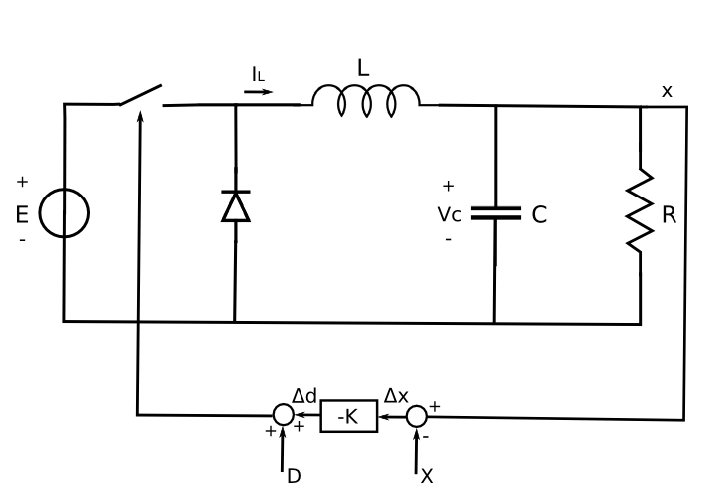
\includegraphics[width=0.55\columnwidth]{figures/nl_models_buck_circuit.eps}
	\caption{Circuito do conversor CC-CC Buck}
	\label{fig:nl_models_buck_circuit}
\end{figure}

Modelos polinomiais n�o resultam em bons modelos para a din�mica de \eqref{eq:nl_alg_buck_circ}. Um
modelo com estrutura {\it{ad rock}}, que aproxima relativamente bem a caracter�stica est�tica do
conversor �: \cite{aguirre_maps}

\begin{equation}
y(t)=O exp\left [ 22-y(t-1) \right ]+ \frac{a\; y(t-1)^2 -b\; y(t-1)+c}{y(t-1)}
\nonumber
\end{equation}

Onde $O=46.429$, $a=2.6204$, $b=99.875$ e $c=1.4171\times 10^3$. Por outro lado a 

Para aplicar o algoritmo, escolhe-se inicialmente um modelo para o sistema em an�lise. O modelo
racional \eqref{eq:nl_alg_buck_rational} aproxima bem a din�mica em quest�o.

\begin{equation}
y(t)=\frac{8.658+0.1223\times10^{-2}y(t-1)^3-0.441\times10^{-1}y(t-1)^2}
{1-0.8381\times10^{-1}y(t-1)+0.1766\times10^{-2}y(t-1)^2}
\label{eq:nl_alg_buck_rational}
\end{equation}

Tendo o modelo escolhido � poss�vel aplicar o algoritmo apresentado na se��o
(\ref{sec:nl_si_algorithms_rationals}). 

Os parametros da equa��o \eqref{eq:nl_alg_buck_rational} s�o os valores de refencia para a utiliza��o do
m�todos descrito em \cite{aguirre}. Utilizando o algoritmo previamente apresentado, o resultado da estimativa
foi:

\begin{equation}
\theta =\begin{bmatrix}
8.8807 & 8.6698\times 10^{-4} &-0.0359 &-0.0736 & 0.0013 
\end{bmatrix}
\nonumber
\end{equation}

Como pode ser observado, pelos resultados de $\theta$ obtidos e os valores esperados, existe polariza��o na
estimativa obtida. Isso em parte se d� pela falta de capacidade da classe de modelos escolhida em representar
o processo real e pela escolha do modelo de r�ido que para este caso foi apenas utilizado o erro da
estimativa, com rela��o a sa�da do sistema real obtido.

Foram utilizadas amostras de 100 pontos para esta estimativa e realizados 100 experimentos de Monte Carlo.
Os resultados obtidos foram de uma m�dia de:

\begin{equation}
\text{m�dia de }\;\theta =\begin{bmatrix}
8.8976  &    8.6762\times 10^{-4}    & -0.0360 &  -0.0736  &  0.0013
\end{bmatrix}
\nonumber
\end{equation}

e uma vari�ncia de

\begin{equation}
\text{vari�ncia }\;\theta =\begin{bmatrix}
0.4842\times 10^{-3}  \\ 1.8004\times 10^{-12} \\ 3.5416\times 10^{-9} \\ 1.9850\times 10^{-9} \\ 2.4100\times
10^{-12}
\end{bmatrix}^T
\nonumber
\end{equation}

com uma covari�ncia de 

\begin{equation}
\text{Covari�ncia de }\;\theta = 1.0\times 10^{-3}\begin{bmatrix}
 0.4842 &  0.0000 & -0.0011 &  0.0007 &-0.0000 \\
 0.0000 &  0.0000 & -0.0000 & -0.0000 & 0.0000 \\
-0.0011 & -0.0000 &  0.0000 & -0.0000 & 0.0000 \\
 0.0007 & -0.0000 & -0.0000 &  0.0000 &-0.0000 \\
-0.0000 &  0.0000 &  0.0000 & -0.0000 & 0.0000 
\end{bmatrix}
\nonumber
\end{equation}

%===============================================================================
\subsection{Outros Exemplos}
\label{sec:nl_si_algorithms_rationals}
%===============================================================================

O sistema descrito abaixo ser� utilizado para a simula��o. 

\begin{equation}
y(k)=\frac{\theta_1y(k-1)+\theta_2y(k-1)u(k-1)+\theta_3u(k-1)}{1+\theta_4y^{2}(k-1)+\theta_5y^{2}(k-2)}
\label{eq:nl_rat_exemple2}
\end{equation}

Para o sistema real utilizou-se os valores de refer�ncia: $\theta= $

\begin{equation}
\theta = 
\begin{bmatrix}
0.2 & 0.1 & 1 & 1 & 1
\end{bmatrix}
\nonumber
\end{equation}

Utilizando par a simula��o um sinal PRBS de 635 pontos e um ru�do de variancia $\sigma^2=0.005$ os resultados
da m�dia de 100 estimativas de Monte Carlo foram:

\begin{equation}
\text{m�dia }\;\theta =\begin{bmatrix}
0.1991  &  0.0995  &  0.9963  &  0.9899  &  0.9912
\end{bmatrix}
\nonumber
\end{equation}

A vari�ncia encontrada foi de:

\begin{equation}
\text{vari�ncia }\;\theta =1.0\times 10^{-4} \begin{bmatrix}
0.0089  &  0.0073  &  0.1082  &  0.7179  &  0.7910
\end{bmatrix}
\nonumber
\end{equation}

E a matriz de covari�ncia �:

\begin{equation}
cov(\theta) =1.0\times 10^{-4} \begin{bmatrix}
    0.0089 & -0.0005 & 0.0112 & 0.0213 & 0.0339 \\
   -0.0005 &  0.0073 & 0.0057 & 0.0220 & 0.0091 \\
    0.0112 &  0.0057 & 0.1082 & 0.2529 & 0.2589 \\
    0.0213 &  0.0220 & 0.2529 & 0.7179 & 0.4987 \\
    0.0339 &  0.0091 & 0.2589 & 0.4987 & 0.7910
\end{bmatrix}
\nonumber
\end{equation}

Utilizando a m�dia das estimativas para simular a sa�da do modelo obtido com o sistema real, obteve-se um
custo:

\begin{equation}
V(\theta)=1.1269\times 10^{-4}
\nonumber
\end{equation}

A fim de melhor ilustrar a estimativa obtida, na Figura \ref{fig:nl_rat_example2} s�o apresentadas as
estimativas dos parametros $\theta_1$ e $\theta_2$ e a elipse de $\chi^2=95\%$.

\begin{figure}[htbp]
	\center
	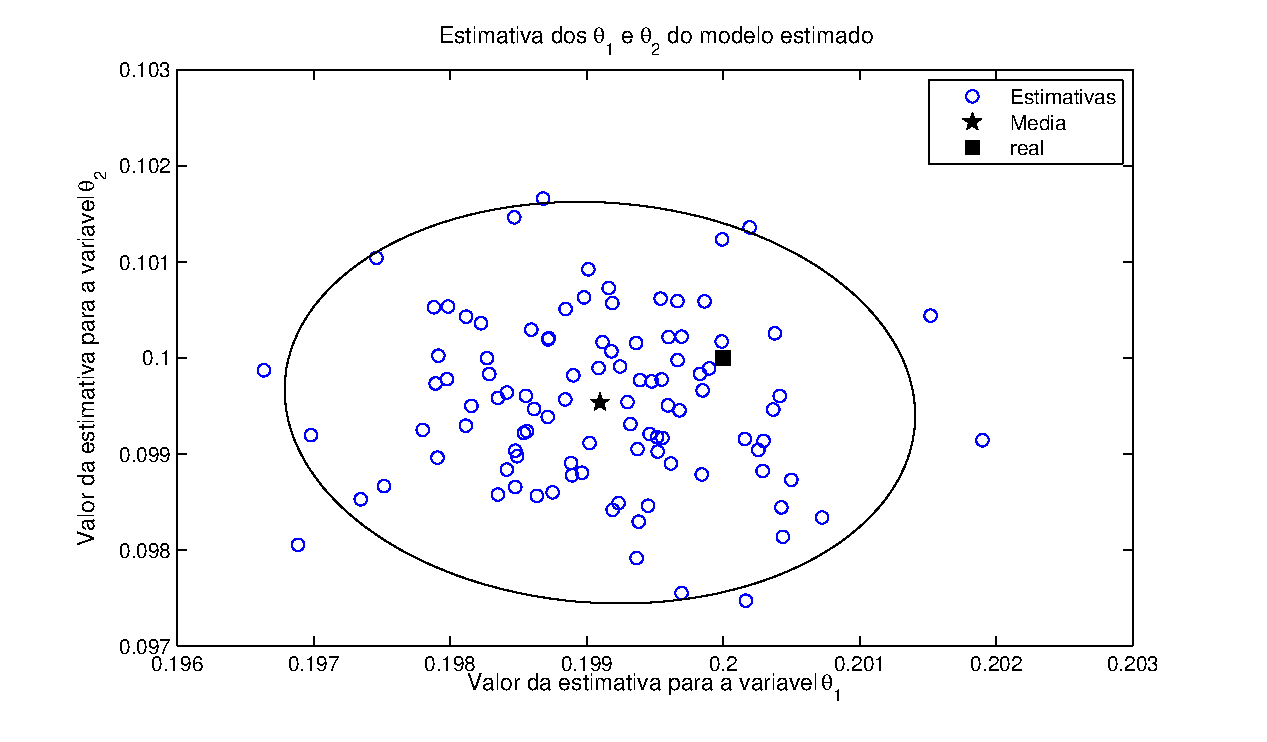
\includegraphics[width=0.9\columnwidth]{figures/rat_example2_a1_a2.eps}
	\caption{Estimativas obtidas nos 100 experimentos de monte carlo realizados para as variavies $\theta_1$ e
	$\theta_2$.}
	\label{fig:nl_rat_example2}
\end{figure}

%===============================================================================
\section{Considera��es Finais}
\label{sec:nl_conclusions}
%===============================================================================


%===============================================================================

